\chapter{Veranderingen die je niet kunt terugdraaien}\label{ch:g5:irreversible-changes}

Er wordt een ei in een hete pan gebroken. Binnen een paar seconden wordt
het heldere, lopende eiwit stevig en wit, en de dooier wordt dikker. Haal
de pan van het vuur, laat het ei afkoelen, zet het in de koelkast: het
wordt nooit meer een rauw ei. Sommige veranderingen kun je terugdraaien
en andere niet. Ze van elkaar onderscheiden is de eerste stap van de
scheikunde.

\begin{recall}
Een vaste stof die in water \omterm{def:g2:mixing-and-dissolving:dissolve}{oplost}, is er nog: als het water opdroogt,
blijft de vaste stof achter (\cref{ch:g2:mixing-and-dissolving}). Bij een
\omterm{def:g4:what-a-fire-needs:burning}{verbranding} ontstaan nieuwe stoffen --- as, rook, koolstofdioxide,
waterdamp --- en de \omterm{def:g4:what-a-fire-needs:fuel}{brandstof} is voorgoed weg
(\cref{ch:g4:what-a-fire-needs}).
\end{recall}

\begin{omfigure}
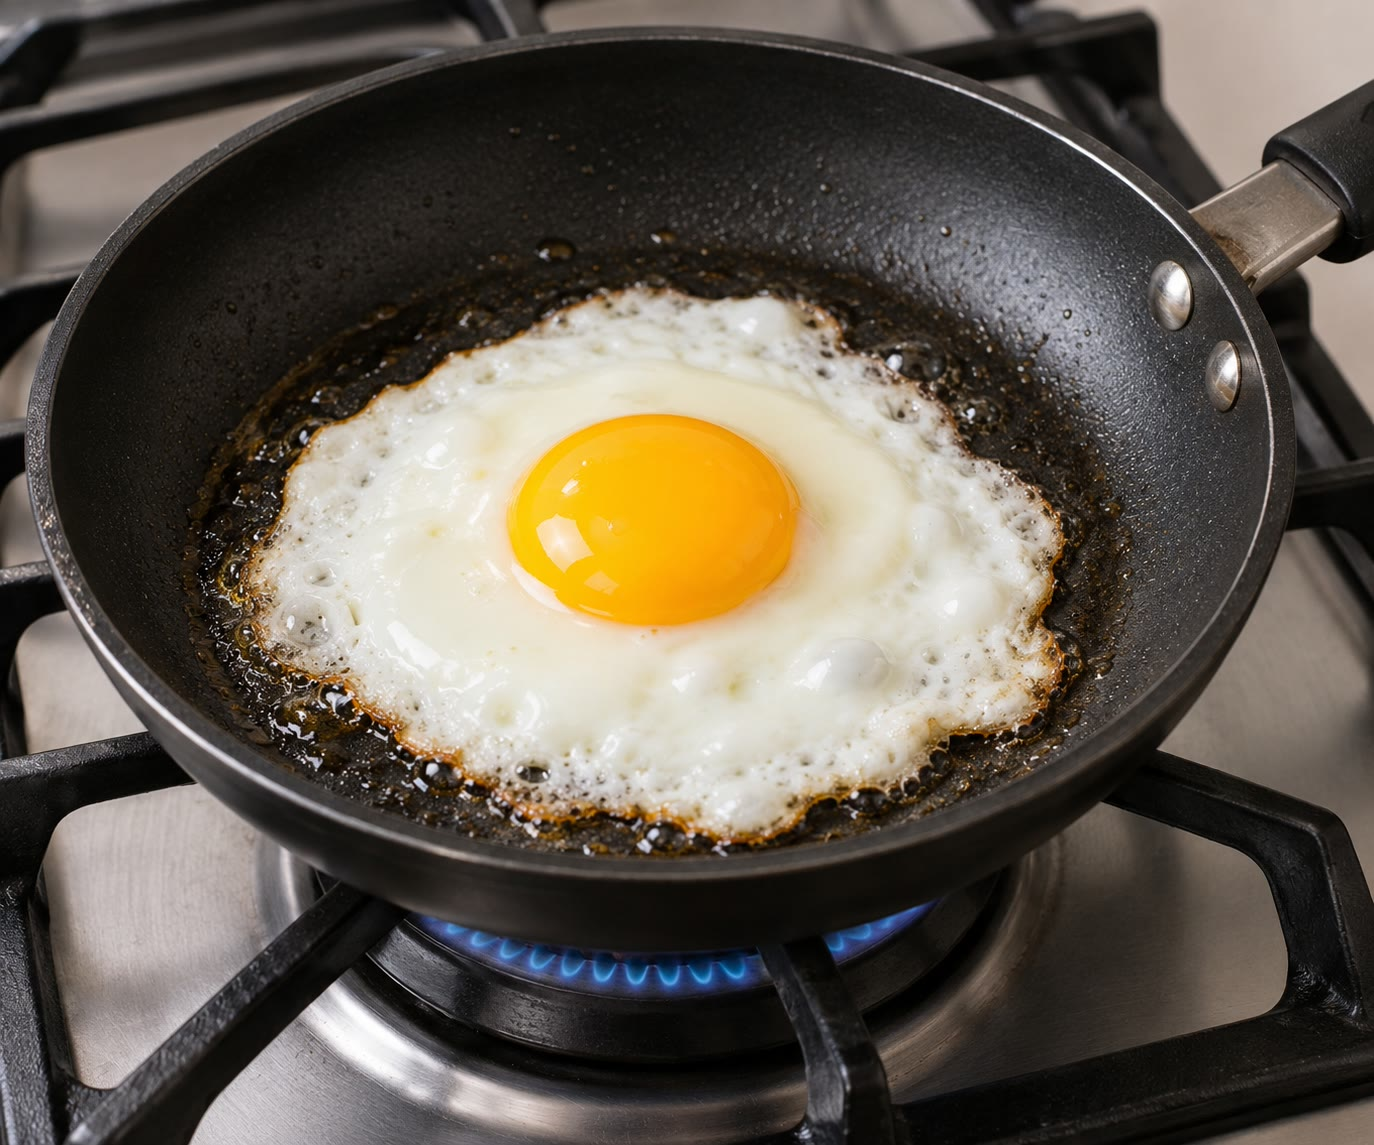
\includegraphics[width=0.55\linewidth]{images/book1/ai/g5-egg-frying.jpg}

{\small Een ei in de koekenpan: het heldere eiwit is stevig en wit
geworden, voorgoed.}
\end{omfigure}

\section{Veranderingen die je kunt terugdraaien}

\begin{definition}[Omkeerbare verandering]\label{def:g5:irreversible-changes:reversible}
Een \emph{omkeerbare verandering}\index{omkeerbare verandering} is een
verandering die je kunt terugdraaien, zodat je precies terugkrijgt waar
je mee begon.
\end{definition}

\begin{example}[Oplossen en opdrogen]\label{ex:g5:irreversible-changes:dissolve}
Suiker die je door water roert, \omterm{def:g2:mixing-and-dissolving:dissolve}{lost op}. Laat het water verdampen, en de
suiker komt terug: dezelfde suiker, net zo zoet als eerst. \omterm{def:g2:mixing-and-dissolving:dissolve}{Oplossen} is
een \omterm{def:g5:irreversible-changes:reversible}{omkeerbare verandering}.
\end{example}

\begin{example}[IJs en water]\label{ex:g5:irreversible-changes:ice}
Een ijsblokje smelt op een warm bord tot water; zet het water in de
vriezer, en het wordt weer ijs. Smelten en bevriezen zijn \omterm{def:g5:irreversible-changes:reversible}{omkeerbare
veranderingen}. (Waarom water smelt en bevriest, staat in het
natuurkundeboek.)
\end{example}

\begin{example}[Mengen]\label{ex:g5:irreversible-changes:mix}
Zand dat met grind gemengd is, kun je weer uit elkaar \omterm{def:g3:separating-mixtures:sieve}{zeven}; modderwater
kun je \omterm{def:g3:separating-mixtures:filter}{filtreren}. \omterm{def:g2:mixing-and-dissolving:mix}{Mengen} is een \omterm{def:g5:irreversible-changes:reversible}{omkeerbare verandering}: er ontstaat niets
nieuws, en de delen kunnen weer gescheiden worden
(\cref{ch:g3:separating-mixtures}).
\end{example}

\section{Veranderingen die je niet kunt terugdraaien}

\begin{definition}[Onomkeerbare verandering en chemische verandering]\label{def:g5:irreversible-changes:chemical-change}
Een \emph{onomkeerbare verandering}\index{onomkeerbare verandering} is
een verandering die je niet zomaar kunt terugdraaien. Bij de meeste
daarvan ontstaan nieuwe stoffen die er aan het begin niet waren: zo'n
verandering heet een \emph{chemische verandering}\index{chemische verandering}.
\end{definition}

\begin{example}[Zes chemische veranderingen]\label{ex:g5:irreversible-changes:six}
\begin{itemize}
  \item \textbf{Een ei bakken}: het lopende, doorzichtige eiwit wordt
        stevig en wit.
  \item \textbf{Een cake bakken}: vloeibaar beslag wordt een luchtige
        cake, bruin aan de buitenkant, met een nieuwe geur.
  \item \textbf{\omterm{def:g4:what-a-fire-needs:burning}{Branden}}: hout wordt as, rook, koolstofdioxide en
        waterdamp.
  \item \textbf{Roesten}: glanzend ijzer dat buiten in de regen blijft
        liggen, raakt bedekt met een bladderende oranjebruine stof, roest.
  \item \textbf{Melk die zuur wordt}: als je melk dagenlang vergeet,
        wordt ze dik, vormt ze klontjes en ruikt ze zuur.
  \item \textbf{Een doorgesneden appel die bruin wordt}: het lichte
        vruchtvlees kleurt binnen een uur bruin aan de \omterm{def:g4:air-a-mixture-of-gases:air}{lucht}.
\end{itemize}
In elk geval is er iets nieuws gemaakt, en is er geen eenvoudige manier
om terug te krijgen waar we mee begonnen.
\end{example}

\begin{omfigure}
\begin{minipage}[t]{0.48\linewidth}\centering
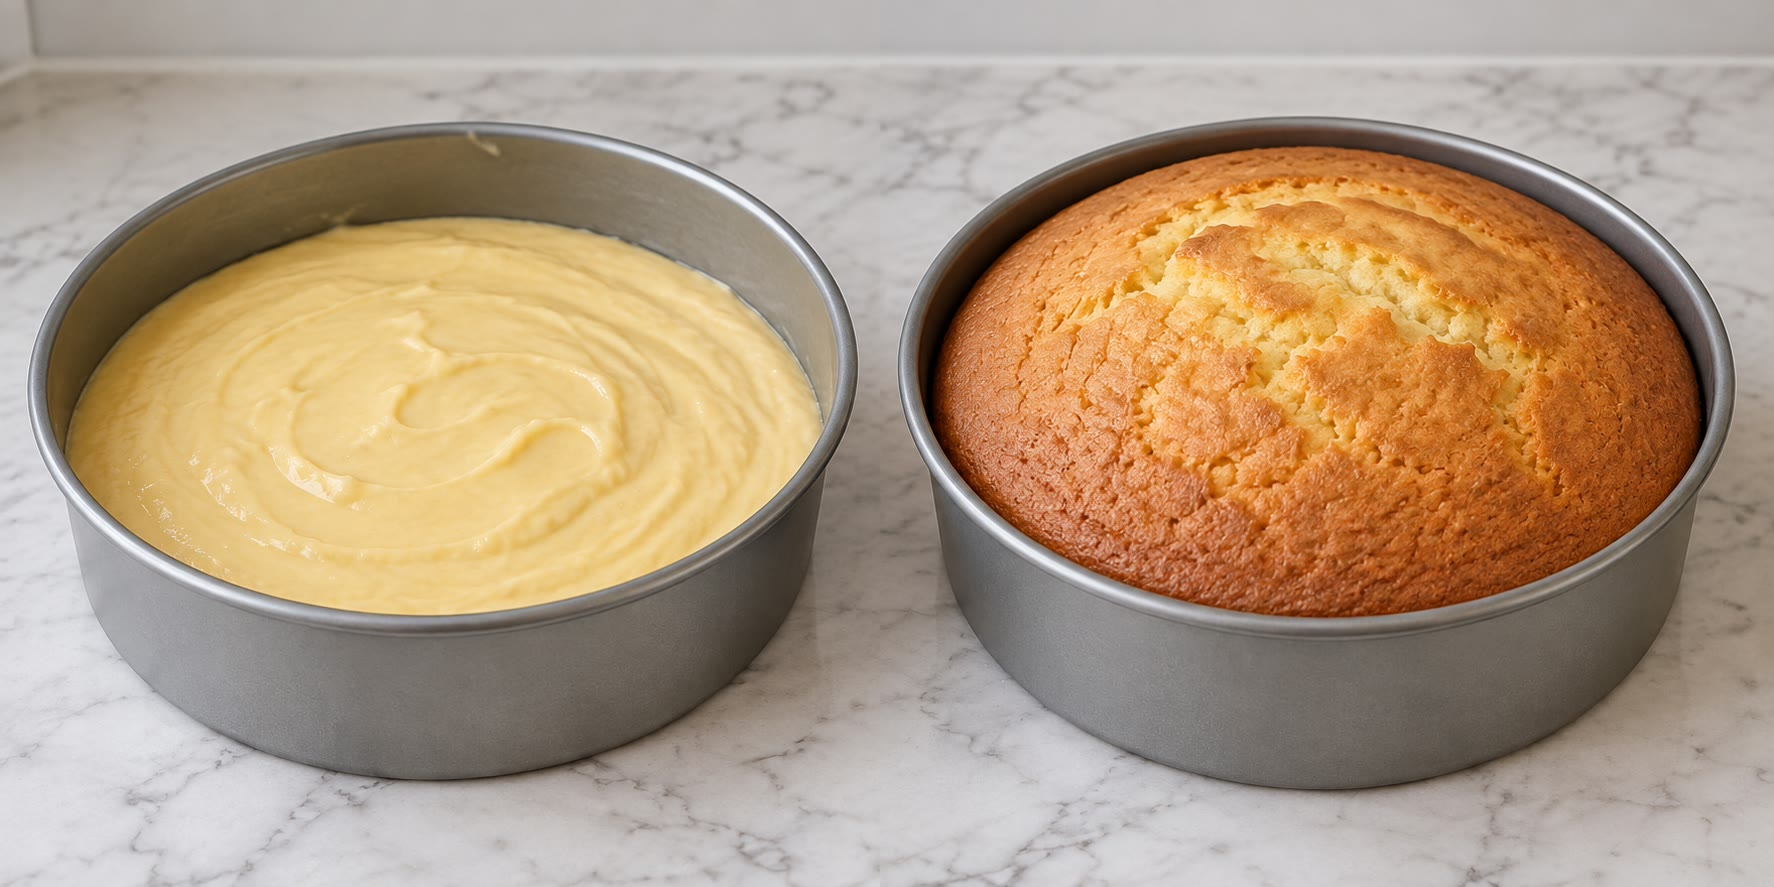
\includegraphics[width=\linewidth,height=4.6cm,keepaspectratio]{images/book1/ai/g5-cake-before-after.jpg}

{\small Eerst beslag, daarna cake: bakken kun je niet terugdraaien.}
\end{minipage}\hfill
\begin{minipage}[t]{0.48\linewidth}\centering
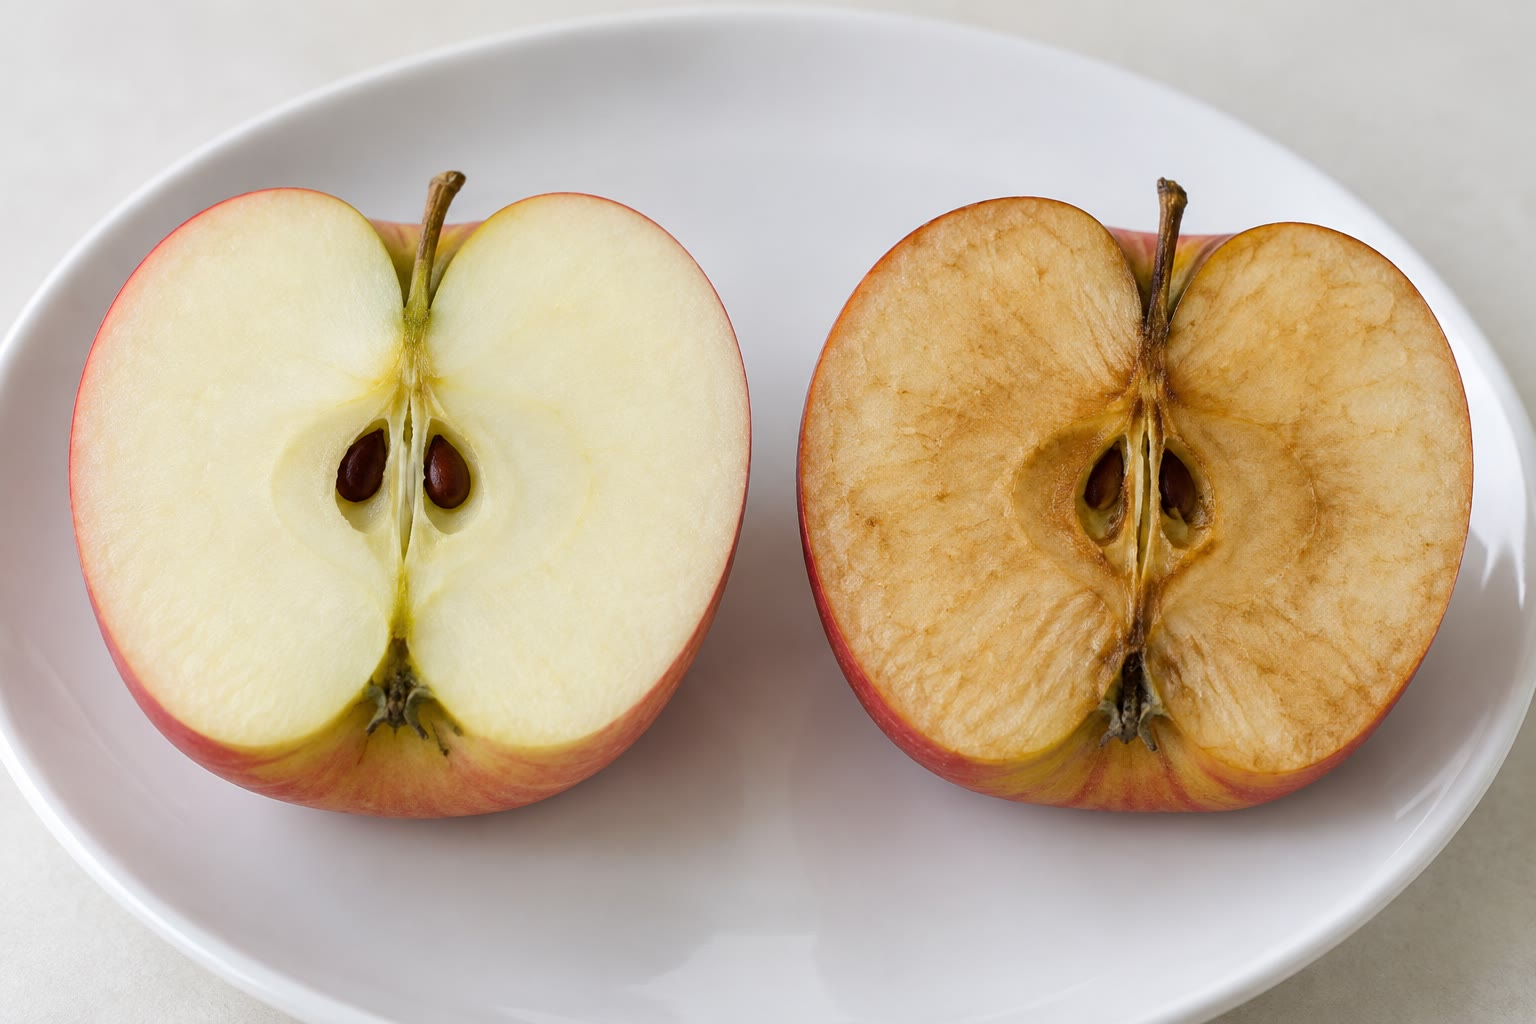
\includegraphics[width=\linewidth,height=4.6cm,keepaspectratio]{images/book1/ai/g5-apple-browning.jpg}

{\small Een verse helft en een helft die een uur aan de \omterm{def:g4:air-a-mixture-of-gases:air}{lucht} heeft
gelegen.}
\end{minipage}
\end{omfigure}

\begin{omfigure}
\begin{tikzpicture}[font=\small]
  \node[font=\small\bfseries, omDef] at (2.7,4.6) {terug te draaien};
  \node[font=\small\bfseries, omProp] at (9.6,4.6) {niet terug te draaien};
  \draw[black!30] (6.1,4.9) -- (6.1,-0.3);
  % reversible pairs
  \foreach \y/\a/\b in {3.6/{suiker + water}/{suikerwater}, 2.0/{ijs}/{vloeibaar water},
                        0.4/{zand + grind}/{een mengsel}} {
    \node[draw=omDef, fill=omDef!6, rounded corners=2pt, minimum width=2.3cm,
      minimum height=0.8cm] at (0.9,\y) {\a};
    \node[draw=omDef, fill=omDef!6, rounded corners=2pt, minimum width=2.3cm,
      minimum height=0.8cm] at (4.6,\y) {\b};
    \draw[->, thick, omDef] (2.3,\y+0.12) -- (3.25,\y+0.12);
    \draw[<-, thick, omDef] (2.3,\y-0.12) -- (3.25,\y-0.12);
  }
  % irreversible ones
  \foreach \y/\a/\b in {3.6/{rauw ei}/{gebakken ei}, 2.0/{hout}/{as, rook, gassen},
                        0.4/{ijzer}/{roest}} {
    \node[draw=omProp, fill=omProp!6, rounded corners=2pt, minimum width=2.0cm,
      minimum height=0.8cm] at (7.6,\y) {\a};
    \node[draw=omProp, fill=omProp!6, rounded corners=2pt, minimum width=2.9cm,
      minimum height=0.8cm] at (11.5,\y) {\b};
    \draw[->, thick, omProp] (8.8,\y) -- (9.85,\y);
  }
\end{tikzpicture}

{\small Links: \omterm{def:g5:irreversible-changes:reversible}{omkeerbare veranderingen}, de dubbele pijl zegt dat ze
twee kanten op kunnen. Rechts: \omterm{def:g5:irreversible-changes:chemical-change}{chemische veranderingen}, maar één kant
op.}
\end{omfigure}

\section{Aanwijzingen dat er een nieuwe stof is ontstaan}

\begin{method}[Is het een chemische verandering? Zoek de aanwijzingen]\label{met:g5:irreversible-changes:clues}
Een nieuwe stof verraadt zich vaak door een van deze aanwijzingen:
\begin{enumerate}
  \item een nieuwe \textbf{kleur} (het bruin van een geroosterde
        boterham);
  \item \textbf{gasbelletjes} die in een vloeistof verschijnen zonder
        dat er verwarmd wordt (azijn op baksoda);
  \item een nieuwe \textbf{geur} (zure melk, aangebrande toast);
  \item er komt \textbf{warmte of licht} vrij (een brandende kaars);
  \item er \textbf{verschijnt een vaste stof} in een heldere vloeistof,
        of er vormen zich klontjes (melk die schift).
\end{enumerate}
Eén aanwijzing alleen kan misleiden: kokend water bruist, maar er
ontstaat niets nieuws --- de belletjes zijn waterdamp, en het water komt
terug als de damp afkoelt. Zoek naar meerdere aanwijzingen, en vraag je
af: kan het worden teruggedraaid?
\end{method}

\begin{omfigure}
\begin{tikzpicture}[font=\small]
  \foreach \k/\t in {0/{nieuwe kleur}, 1/{gasbelletjes}, 2/{nieuwe geur},
                     3/{warmte of licht}, 4/{er komt een vaste stof}} {
    \begin{scope}[xshift=\k*3.2cm]
      \draw[omProp, line width=0.8pt, fill=omProp!5] (0,0) circle (1.0);
      \node[anchor=north, align=center] at (0,-1.15) {\t};
    \end{scope}
  }
  % 1: colour, a slice of toast half brown
  \fill[yellow!20, draw=brown!60] (-0.55,-0.5) rectangle (0.55,0.55);
  \fill[brown!55] (0,-0.5) rectangle (0.55,0.55);
  % 2: bubbles in a beaker
  \begin{scope}[xshift=3.2cm]
    \pic[transform shape, scale=0.45] at (0,-0.55) {beaker={0.7}{omWater!80}};
    \foreach \x/\y in {-0.15/-0.2,0.1/0.05,-0.05/0.25,0.18/-0.35,-0.2/0.15}
      \draw[black!55] (\x,\y) circle (0.05);
  \end{scope}
  % 3: smell, wavy lines
  \begin{scope}[xshift=6.4cm]
    \foreach \x in {-0.35,0,0.35} \draw[black!55, line width=0.8pt, decorate,
      decoration={snake, amplitude=1.5pt, segment length=6pt}] (\x,-0.6) -- (\x,0.6);
  \end{scope}
  % 4: a flame
  \begin{scope}[xshift=9.6cm]
    \fill[orange!80] (0,-0.6) .. controls (-0.45,-0.05) and (-0.15,0.35) .. (0,0.7)
      .. controls (0.15,0.35) and (0.45,-0.05) .. (0,-0.6);
    \fill[yellow!80] (0,-0.45) .. controls (-0.2,-0.1) and (-0.08,0.15) .. (0,0.3)
      .. controls (0.08,0.15) and (0.2,-0.1) .. (0,-0.45);
  \end{scope}
  % 5: solid settling in a test tube
  \begin{scope}[xshift=12.8cm]
    \pic[transform shape, scale=0.4] at (0,-0.65) {testtube={0.75}{omWater!80}};
    \fill[white, draw=black!40] (-0.08,-0.62) rectangle (0.08,-0.5);
    \foreach \x/\y in {-0.04/-0.3,0.04/-0.1,0/0.1} \fill[black!35] (\x,\y) circle (0.03);
  \end{scope}
\end{tikzpicture}

{\small Vijf aanwijzingen dat er misschien een \omterm{def:g5:irreversible-changes:chemical-change}{chemische verandering} is
gebeurd.}
\end{omfigure}

\begin{inthelab}[Azijn op baksoda]
De docent doet een lepel baksoda, een wit poeder, onder in een bekerglas
en giet er wat azijn bij. Het mengsel bruist en schuimt meteen op: er
ontsnapt een gas, een aanwijzing voor een \omterm{def:g5:irreversible-changes:chemical-change}{chemische verandering}. Als het
bruisen ophoudt, is de baksoda verdwenen, en door opdrogen krijg je die
niet meer terug.
\end{inthelab}

\begin{omfigure}
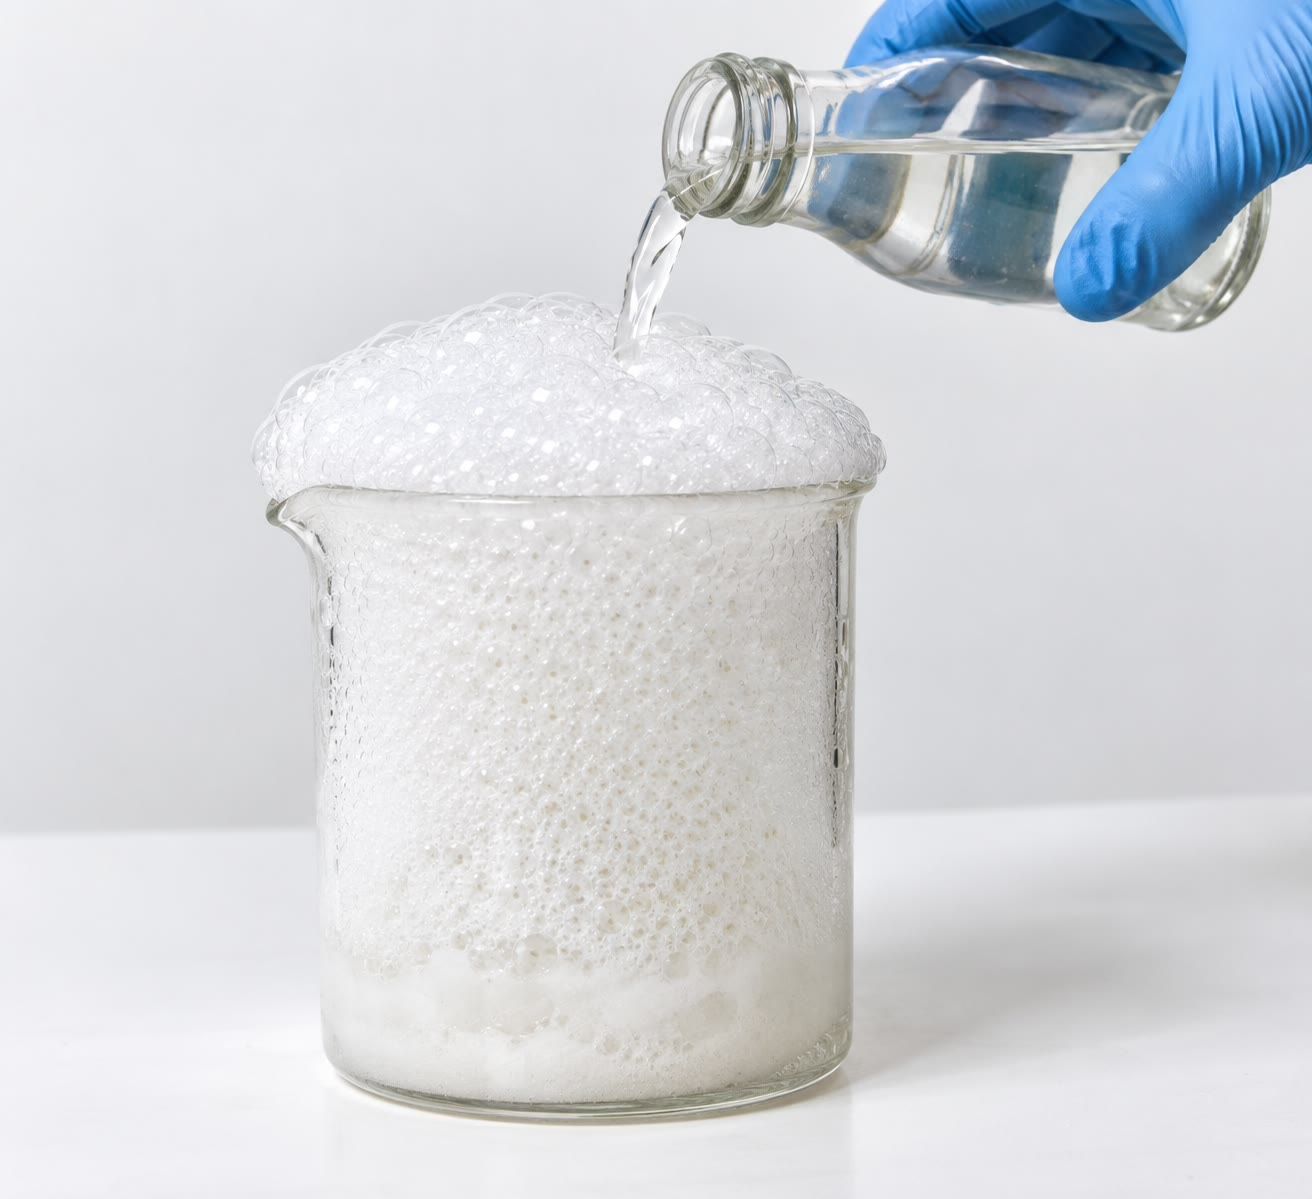
\includegraphics[width=0.5\linewidth]{images/book1/ai/g5-baking-soda-lab.jpg}

{\small Azijn op baksoda: er ontsnapt een gas.}
\end{omfigure}

\section{Nuttige en schadelijke veranderingen}

\begin{proposition}[Chemische veranderingen om ons heen]\label{prop:g5:irreversible-changes:around}
Veel \omterm{def:g5:irreversible-changes:chemical-change}{chemische veranderingen} zijn nuttig: eten koken, brood bakken, gas
\omterm{def:g4:what-a-fire-needs:burning}{verbranden} om een huis te verwarmen, gips of cement dat hard wordt.
Andere richten schade aan: ijzer dat roest, eten dat bederft, hout dat
rot. We kunnen ze niet terugdraaien, maar we kunnen ze wel vertragen:
\begin{itemize}
  \item eten blijft langer goed in de kou van een koelkast;
  \item verf of een laagje olie houdt \omterm{def:g4:air-a-mixture-of-gases:air}{lucht} en water weg van ijzer;
  \item een doorgesneden appel met wat citroensap erover wordt
        langzamer bruin.
\end{itemize}
\end{proposition}

\begin{omfigure}
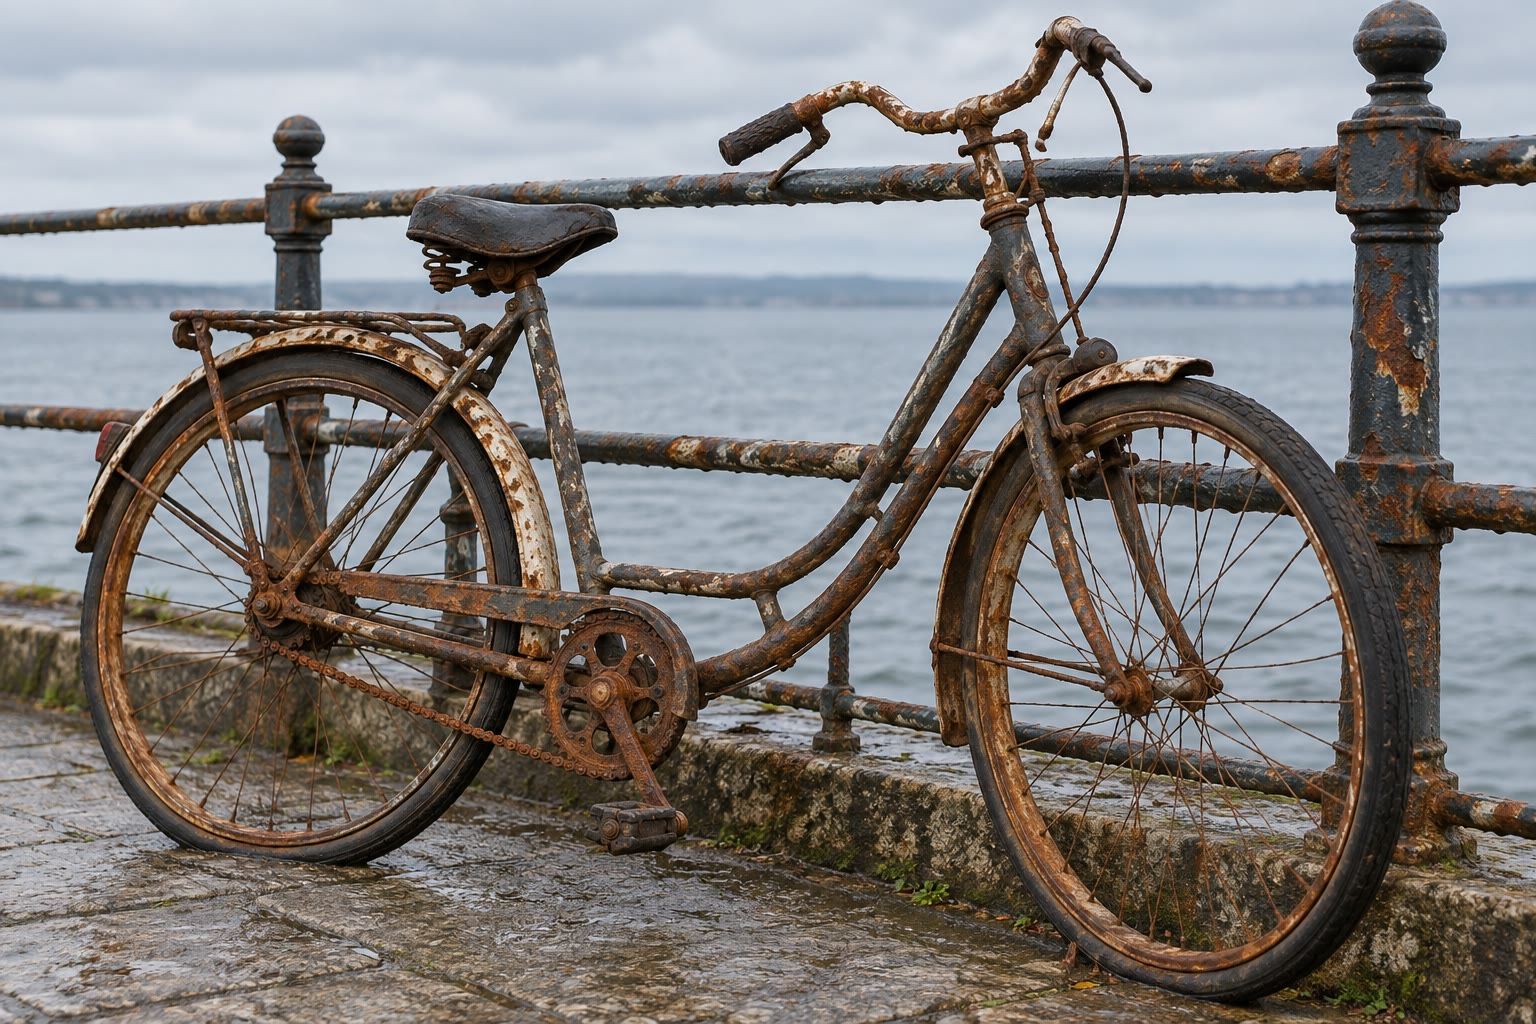
\includegraphics[width=0.55\linewidth]{images/book1/ai/g5-rusty-bicycle.jpg}

{\small Een fiets die jarenlang buiten in de regen heeft gestaan: het
ijzer is geroest.}
\end{omfigure}

\begin{remark}[Terug te draaien, maar niet zomaar]\label{rem:g5:irreversible-changes:not-simply}
``Niet terug te draaien'' betekent dat er geen eenvoudige weg terug is,
zoals afkoelen of opdrogen. Scheikundigen kunnen roest soms weer in
ijzer omzetten, maar alleen met een hoogoven en nieuwe stoffen: dat is
weer een \omterm{def:g5:irreversible-changes:chemical-change}{chemische verandering}, geen terugdraaien.
\end{remark}

\section{Oefeningen}

\begin{exercise}[$\star$]\label{exo:g5:irreversible-changes:1}
Zeg van elke verandering of je ze kunt terugdraaien: chocolade smelten,
een lucifer \omterm{def:g4:what-a-fire-needs:burning}{verbranden}, zout in water \omterm{def:g2:mixing-and-dissolving:dissolve}{oplossen}, brood roosteren.
\end{exercise}

\begin{exercise}[$\star$]\label{exo:g5:irreversible-changes:2}
Wat is een \omterm{def:g5:irreversible-changes:chemical-change}{chemische verandering}? Geef twee voorbeelden uit de keuken.
\end{exercise}

\begin{exercise}[$\star$]\label{exo:g5:irreversible-changes:3}
Zout wordt in water opgelost. Hoe krijg je het zout terug? Is \omterm{def:g2:mixing-and-dissolving:dissolve}{oplossen}
een \omterm{def:g5:irreversible-changes:reversible}{omkeerbare verandering}?
\end{exercise}

\begin{exercise}[$\star$]\label{exo:g5:irreversible-changes:4}
Welke aanwijzingen voor een \omterm{def:g5:irreversible-changes:chemical-change}{chemische verandering} merk je als melk zuur
wordt? Noem er twee.
\end{exercise}

\begin{exercise}[$\star$]\label{exo:g5:irreversible-changes:5}
Kijk naar de figuur met de twee kolommen. Welke veranderingen hebben een
dubbele pijl? Wat betekent de dubbele pijl?
\end{exercise}

\begin{exercise}[$\star$]\label{exo:g5:irreversible-changes:6}
Waarom wordt een fietsketting geolied? Welke \omterm{def:g5:irreversible-changes:chemical-change}{chemische verandering}
vertraagt de olie?
\end{exercise}

\begin{exercise}[$\star$]\label{exo:g5:irreversible-changes:7}
Als je azijn op baksoda giet, bruist het. Welke aanwijzing is dat?
\end{exercise}

\begin{exercise}[$\star$]\label{exo:g5:irreversible-changes:8}
Noem een nuttige en een schadelijke \omterm{def:g5:irreversible-changes:chemical-change}{chemische verandering}.
\end{exercise}

\begin{exercise}[$\star$]\label{exo:g5:irreversible-changes:9}
Waarom bewaren we melk in de koelkast?
\end{exercise}

\begin{exercise}[$\star\star$]\label{exo:g5:irreversible-changes:10}
Water bruist als het kookt. Is koken een \omterm{def:g5:irreversible-changes:chemical-change}{chemische verandering}? Leg uit
waarom één aanwijzing niet genoeg is.
\end{exercise}

\begin{exercise}[$\star\star$]\label{exo:g5:irreversible-changes:11}
Tom zegt: ``Als de kaars brandt, smelt het kaarsvet gewoon weg, net als
ijs.'' Gebruik twee aanwijzingen om uit te leggen waarom een brandende
kaars een \omterm{def:g5:irreversible-changes:chemical-change}{chemische verandering} is, en niet alleen smelten.
\end{exercise}
